\section{Results}

Like for animals \cite{}, hunter-gatherers \cite{}, and human mobility in modern environments \cite{}, we find that human mental search follows a L\'evy flight pattern, and more precisely a continuous time random walk (CTRW) \cite{montroll_random_1965}, which is defined by a heavy-tailed distribution of displacement, 

\begin{equation}
\label{displacements}
pdf(\Delta r) = \Delta r^{-\alpha -1},
\end{equation}

and by a heavy-tailed distribution of waiting times before the next move, 

\begin{equation}
\label{wtimes}
pdf(\Delta t) = \Delta t^{-\beta -1}.
\end{equation}

For both treatment 1 and 2, the characteristic parameters $\alpha$ and $\beta$ appear to be similar. $\alpha = 0.40(5)$ (see Figure \ref{fig:CTRW}A), and the probability density function of waiting times exhibits 2 regimes:  $\beta_{\Delta t < 125} = 0.38(4)$ and $\beta_{\Delta t > 125} = 1.59(5)$ (see Figure \ref{fig:CTRW}B). Incremental displacement is measured as the XXXX distance between 2 solutions proposed by the participant (see SI).

\begin{figure}[h!]
\begin{center}
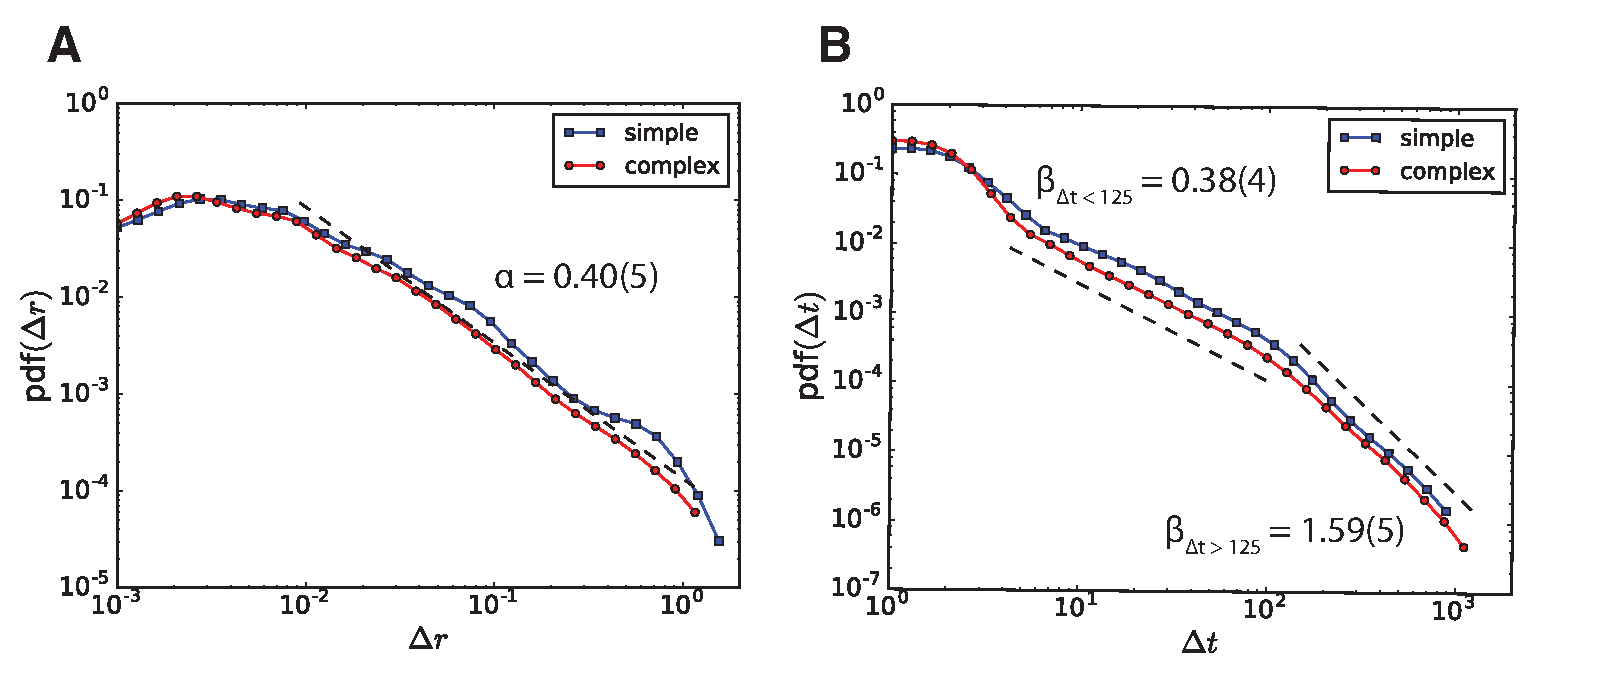
\includegraphics[width=17cm]{figures/CTRW.eps}
\caption{\footnotesize{{\bf A.} Probability density function of displacement $pdf(\Delta r) = \Delta r^{-\alpha -1}$ with $\alpha = 0.40(5)$ with a cut-off limited by the largest possible displacement, which is $\sqrt{k}$ with $k$ the number of conditional probabilities to evaluate. {\bf B.}  Probability density function of waiting time $pdf(\Delta t) = \Delta t^{-\beta -1}$ with 2 regimes : $\beta_{\Delta t < 125} = 0.38(4)$ and $\beta_{\Delta t > 125} = 1.59(5)$. Distributions of $\Delta r$ and $\Delta t$ are equivalent for the simple and complex treatments.}}
\label{fig:CTRW}
\end{center}
\end{figure}

These results alone would suggest a super-diffusive search process, with mean square displacement (MSD) predicted to be,

\be
prediction_msd.
\ee

%$\sim t^{\mu}$ with  $\mu_{Levy} = 1$ \
%or super-diffusion $\mu_{CTRW} = \beta$ \cite{21,23}). Here, however, mean square displacement (MSD) decays as $\sim t^{\mu}$ with $\mu_{simple} =-0.23(2)$ and $\mu_{complex} =-\
%0.26(1)$ showing a much slower convergence than is generally expected.

However, the observed $MSD  =  XX$ rather exhibits a sub-diffusive process (see Figure \ref{}X for a comparison), hence suggesting a more subtle mental search, compared to a search process, which would not optimize through the progressive integration of information \cite{} and use of memory \cite{}. We shall emphasize that the distribution of excursions is much more heavy-tailed than what has been computed as optimal search for foraging (i.e., $\alpha \approx 1$\cite{viswanathan_optimizing_1999,reynolds_displaced_2007,viswanathan_physics_2011}). \\

{\bf [A note on waiting times $\rightarrow$ maybe in discussion ?]} Note that waiting times  have been observed \cite{humphries_optimal_2014,song_modelling_2010}\\


{\bf [the subsection on performance could be here]}


We shall analyze the ``anomalous" mental search process, proceed to the identification of deviations from the ``optimal search" process (i.e., $\alpha = 1$). These deviations are (i) a much smaller power law exponent compared to other findings (ballistic process) and (ii) a much smaller (sublinear) MSD, which seems to contradict the ballistic process, which stems from $\alpha = 0.4 < 1$. 

Several mechanisms of cognition may explain such inconsistency.  Optimal foraging does not account for incentives \cite{}, continuous information intake \cite{}, memory \cite{}, information processing \cite{}, and cognitive biases that may hinder the mental search process \cite{}. 


\subsection{Exploration beyond currently known solution space vs. optimization from current knowledge}

When participants start, they have an abstract view, yet no experience, of the whole solution space (i.e., they know that they must find values between 0 and 1 for 8 (resp. 16) parameters for treatment 1 (resp. treatment 2). Exploring beyond the already known solution space (i.e., convex hull {\bf [define if not done previously)]}) is critical {\bf [how much critical is it ? very important question to be settled]}.

We are interested in proposed models, which go beyond the solution space known at iteration $i$. If twice $\langle D_{jsd,i} \rangle$, the average distance of solution $j$ compared to all previous solutions $i < j$, is larger than $ max(D_{jsd})$ the maximum distance between 2 solutions in $iterations = \{1,...,i\}$, then the new proposed model {\it {\bf incorporates causal hypotheses and conditional independence assumptions, which are not entailed by previously explored models}} and contributes to the enlargement of the currently explored joint-hypotheses space. To measure how much a proposed model is explorative, versus exploitative of causal and conditional independence structures, we define the ratio:

\begin{equation}
EE_{j} = \frac{2 \langle D_{jsd,j} \rangle}{max(D_{jsd,1,...,j})}.
\end{equation}

For $EE < 1$, the individual is choosing an exploitative solution, that lies within the boundaries of the convex hull of already explored solutions. For $EE \approx 1$, the proposed solution is on -- or close to -- the boundaries, and for $EE > 1$, the proposed solution is outside the convex hull, and therefore explorative. The larger $EE$, the more explorative the proposed solution. For both 3-node and 4-node BN treatments,  the number of explorative moves is over all people much larger than exploitative ones :  $5416$ vs. $1873$ (resp. $6260$ vs. $4689$). It is of course critical to know how exploration and exploitation vary over time. It is optimal, in fact necessary to explore a lot in the beginning, when not much is known about the space or its payoffs, but it is diminishingly fruitful to explore towards the end of the game, for three reasons: 1) because towards the end it is harder to find truly new solutions as one's creativity is more taxed to find further unexplored patterns, 2) because it may seem less likely that the novel solutions--once they are found--will be improvements and 3) because even if improvements are as likely as losses, it is harder to make up for losses towards the end and thus risk is affected. The structure here is as in a work-retirement game wherein it makes sense to speculate and take large risks earlier in one's career when the benefits can have immense impacts on one's whole life span and it makes sense to be conservative later in one's career, where losses can not be easily made up for and most of the opportunities appear to have already been considered, whether this is truly the case or it is just a tired loss of attention towards the end.    
%{\bf yes! I very much agree and one could in fact work out some equilibrium or optimal exploration as a function of time and cognitive costs as well as expected benefit from exploration (itself perhaps subject of experiential learning and a model of its own) ...I'm not saying that we should, but we may mention it as a possibility of something that an economist, or a theorist of incentivized optimal learning might be interested in doing. }

An exact equilibrium path of allocation between exploitation and exploration could be worked out, that logically should start with maximum and speedy exploration of the space--exactly as speedily as hypotheses can be tested with new observations and not speedier.  This speedy exploration should be the policy in the beginning, when the mental state is complete ignorance.  The game should end in coming as close as possible to understanding the process, such that any risk of further exploration is no longer worth the expected life-time benefits and exploration should completely stop. This is the time when optimization should be completely exploitative fine-tuning.    
 



\begin{figure}[h!]
\begin{center}
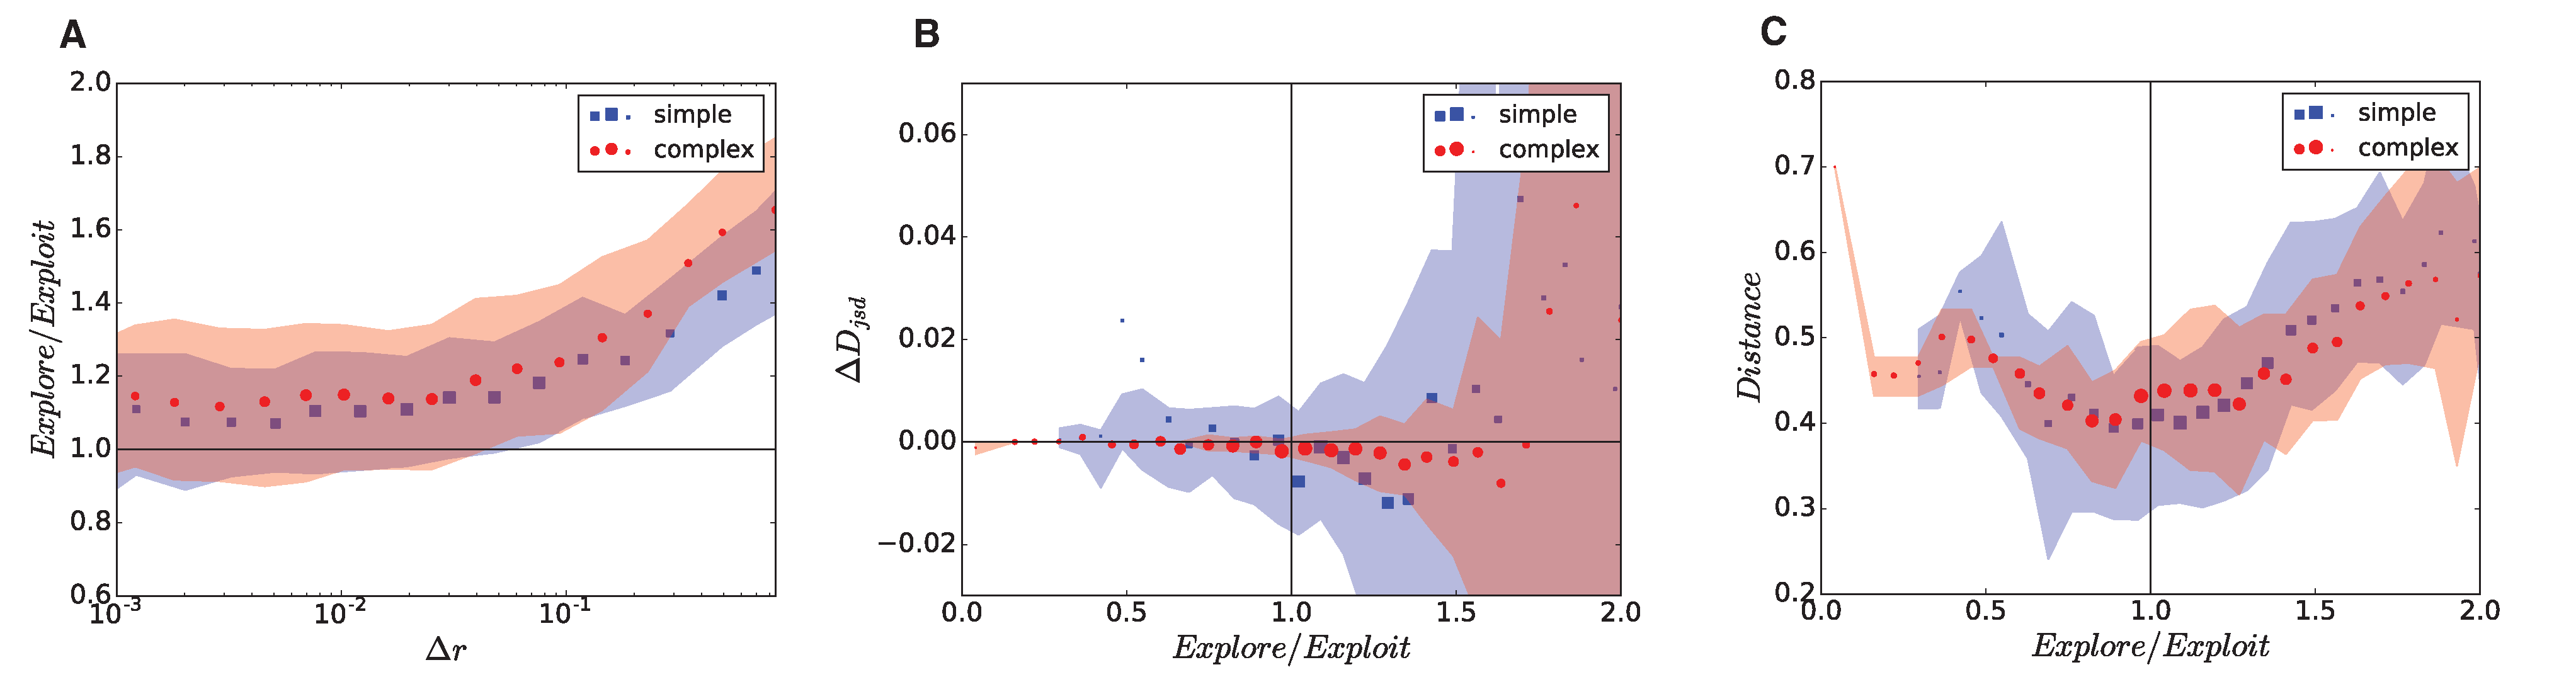
\includegraphics[width=18cm]{figures/EE.eps}
\caption{{\bf A.} Explore / Exploit ($EE$ )as a function of displacement $\Delta r$. {\bf B.} $\Delta D_{jsd}$ as a function Explore / Exploit: Improvement seems better for $EE \approx 1.4$. {\bf C.} $D_{jsd}$ as a function of $EE$: As distance gets smaller, a balance around $EE = 1$ seems to be reached.}
\label{fig:pdf_return}
\end{center}
\end{figure}

\subsection{Return to previously visited sites}
We also find that individuals tend to repeatedly return to previously visited solutions. The probability distribution is found to follow a power law with exponent $\gamma \approx 1.5$  (see Figure \ref{fig:memory}B)

\subsection{Recency of memory}
Memory plays a central role in recombining multiple previously explored models into new ones. We find strong influence of a focal model on subsequent models. On average over all participants in each treatment, influence $I$ decays as $I \sim t^{-\chi}$ with $\chi = 0.48(2)$ ($p < 0.01$ and $R > 0.32$)  (Figure \ref{fig:2}B). Because the time decay exhibits a power law with exponent $\chi < 1$, on average, models proposed in the past never vanish from memory, and may be reused or inspire future models. If we assume that the rate of proposed models remains roughly constant  over time for some participant, as time passes it gets statistically harder to come up with novel solutions ``because mental constructions are imprinted by past experience'' and the cognitively low hanging fruits as well as all of their combinations are being used up, leaving less and less intuitive solutions in the unexplored space of models. Often--as in the Monty Hall example--the true processes of stochastic influence and their observational consequences are highly counter-intuitive.  


\begin{figure}[h!]
\begin{center}
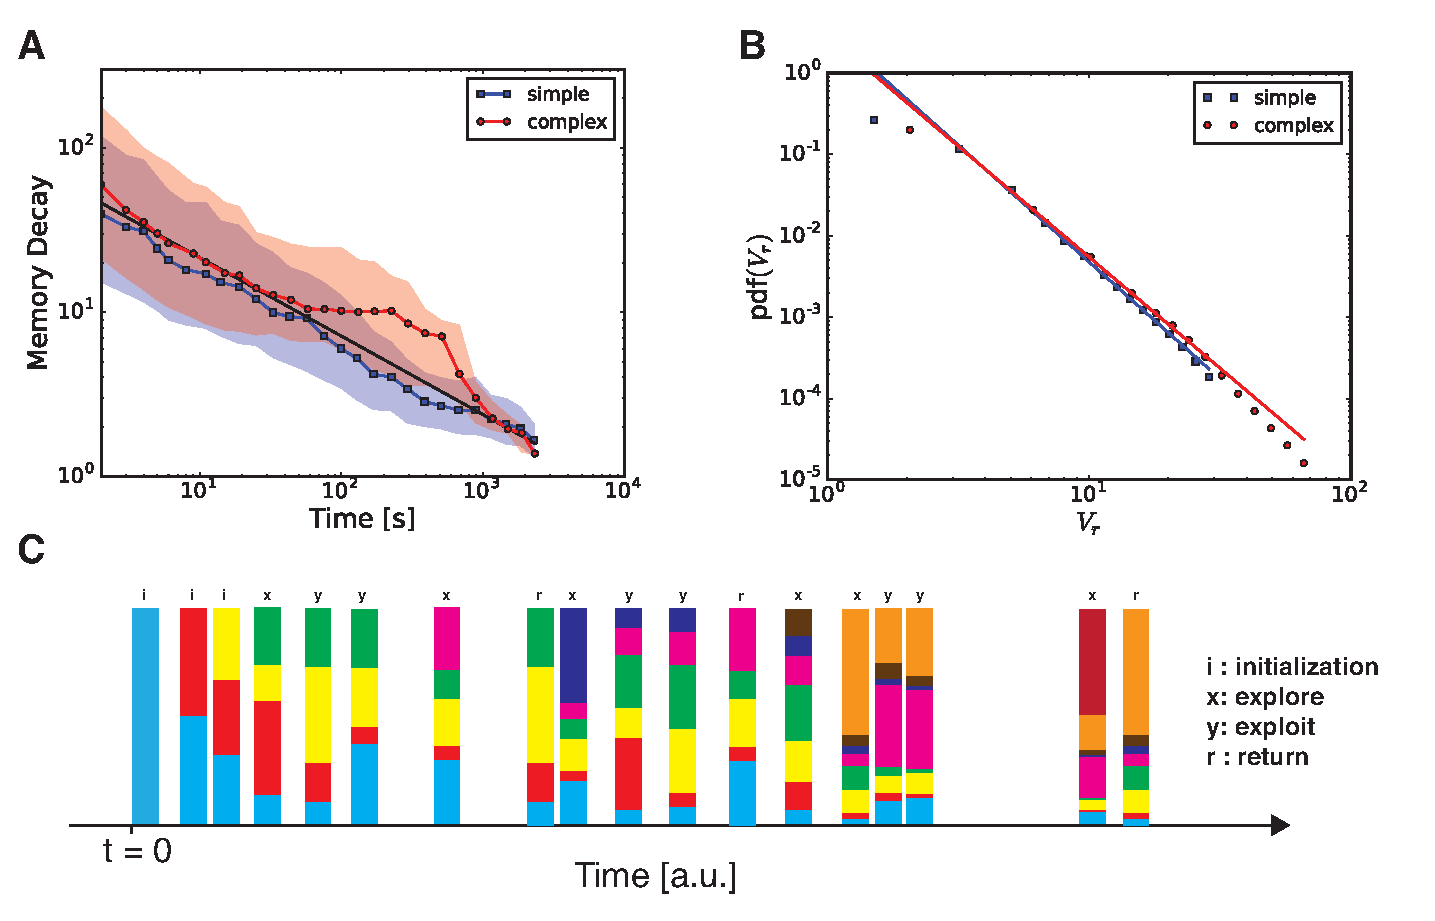
\includegraphics[width=15cm]{figures/memory.eps}
\caption{{\bf A.} Influence of a model proposed at time in subsequent models. The influence is computed as 1/distance between the focal model and subsequent models. On average over all participants in each treatment, influence $I$ decays as $I \sim t^{-\chi}$ with $\chi = 0.48(2)$ ($p < 0.01$ and $R > 0.32$). This result shows that memory is a long memory process, with implications for the convergence to. {\bf B.} Return to previously visited sites : $\mathrm{pdf}(V_r) \sim {V_r}^{- \gamma -1}$, with $\gamma_{simple} = 1.6(1)$ and $\gamma_{complex} = 1.5(1)$ $\rightarrow$ tendency to return to previously visited sites : This goes against the imperative to visit new sites (maximize $S_T$) in order to reduce $D_{min}$ (c.f. Figures \ref{fig:Dmin_vs_St}B and \ref{fig:Dmin_vs_St}C). Moreover, given the large number of sites [$10^{8}$ (resp. $10^{16}$) in the simple (resp. complex) case], it is remarkable that participants tend to return to exactly the same (tiny) spots. This suggest some stickiness of memory. {\bf C.}  Schematic representation of remix dynamics. The color bars show the proportion (i.e., $1/d$) of previously proposed solutions in solution proposed at time $t$. New colors are introduced 	tosignal exploration. From time to time, individuals return to previously visited solutions (signaled by $r$).}
\label{fig:memory}
\end{center}
\end{figure}


\clearpage


%\begin{figure}[h!]
%\begin{center}
%%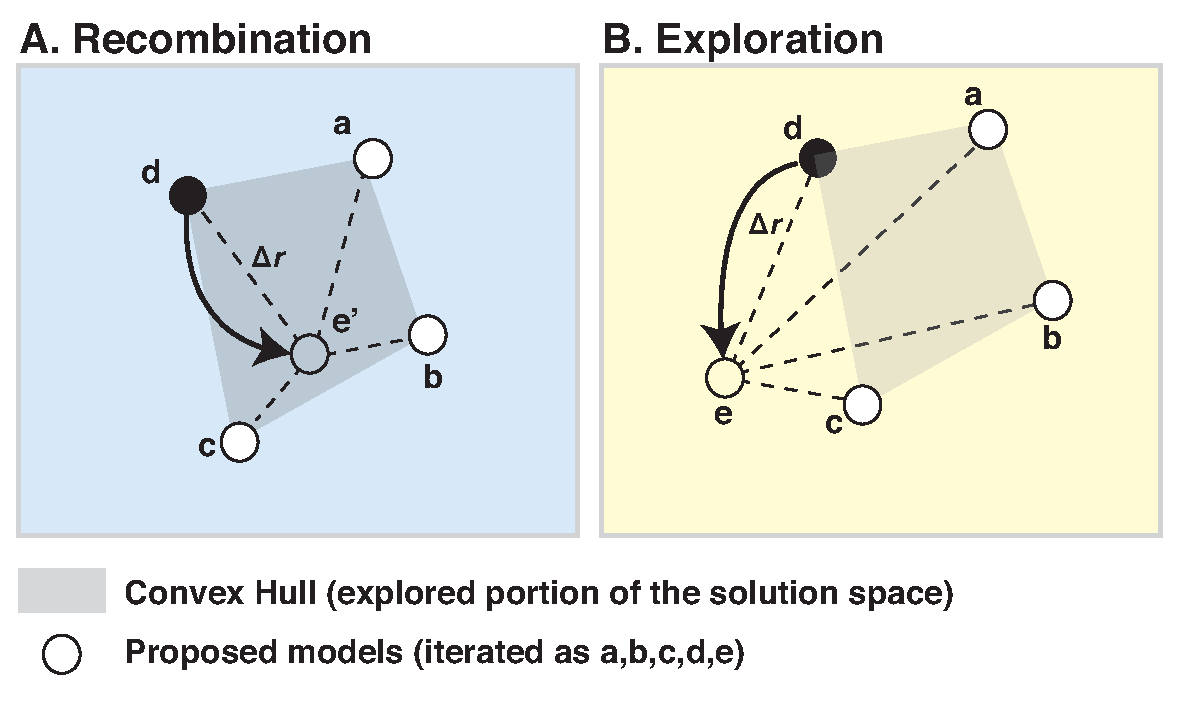
\includegraphics[width=12cm]{figures/figure2.eps}
%\caption{\footnotesize{move patterns}}
%\label{fig:move_patterns}
%\end{center}
%\end{figure}



%{\bf A.} Average Jensen-Shannon Distance $\langle D \rangle$ decays as a function of time as $\sim t^{\nu}$ with $ \nu \approx -0.15(1)$ indicating a very slow convergence to the true model {\bf [indicate $t_0$s and what their values may mean]}. 

%\begin{figure}[h!]
%\begin{center}
%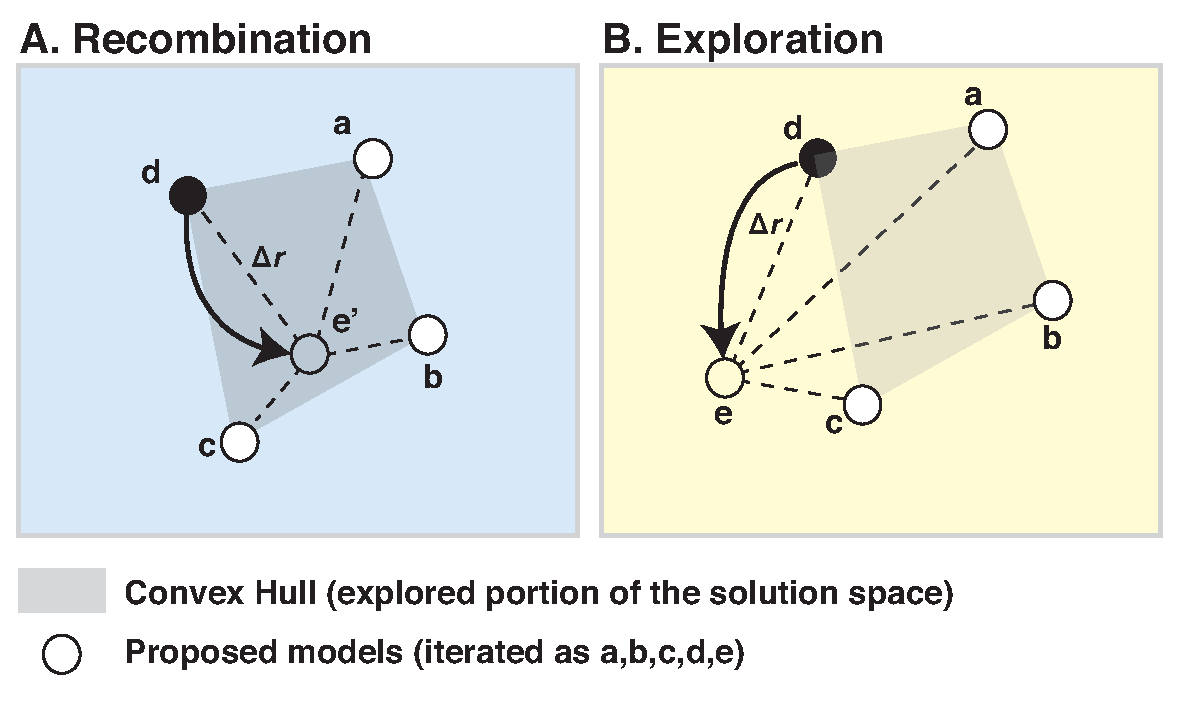
\includegraphics[width=12cm]{figures/figure2.eps}
%\caption{\footnotesize{Simplified diagram of exploration and recombination on a plane: {\bf A. Recombination:} iteration {\bf e'} does not incorporate new information. It is a convex combination of all previous proposed solutions (i.e., $\{a,b,c,d\}$).  {\bf B. Exploration:} the average distance between iteration {\bf e} and all previous iterations is larger than half of the maximum distance between any previous proposed solutions. Exploration is not memoryless: {\bf e} is closer to {\bf c} and {\bf d} than {\bf a} and {\bf b}. }}
%\label{fig:2}
%\end{center}
%\end{figure}


%\subsection{Memory, Return to previously visited sites \& Recombination}


%\begin{figure}[h!]
%\begin{center}
%%\includegraphics[width=16cm]{figures/Figure1.eps}
%\caption{\footnotesize{{\bf A.} return to previously visited sites : $\mathrm{pdf}(V_r) \sim {V_r}^{- \gamma -1}$, with $\gamma_{simple} = 1.6(1)$ and $\gamma_{complex} = 1.5(1)$ $\rightarrow$ tendency to return to previously visited sites : This goes against the imperative to visit new sites (maximize $S_T$) in order to reduce $D_{min}$ (c.f. Figures \ref{fig:Dmin_vs_St}B and \ref{fig:Dmin_vs_St}C). Moreover, given the size of the parameter space [the simplex of dimension $10^{8}$ (resp. $10^{16}$) in the simple (resp. complex) case], it is remarkable that participants tend to return to exactly the same infinitesimal spots in this space. This suggest memory dependent stickiness. {\bf B.} Influence of a model proposed at some time, $t$ in subsequent models at some $t +s$, with $s \geq 1$. The influence is computed as 1/distance between the focal model and subsequent models. On average over all participants in each treatment, influence $I$ decays as $I \sim t^{-\chi}$ with $\chi = 0.48(2)$ ($p < 0.01$ and $R > 0.32$). This result shows that the importance of a memory decays slowly, with implications for the convergence of beliefs to the processes that are the content of those beliefs.}}
%\label{fig:3}
%\end{center}
%\end{figure}

\begin{figure}[h!]
\begin{center}
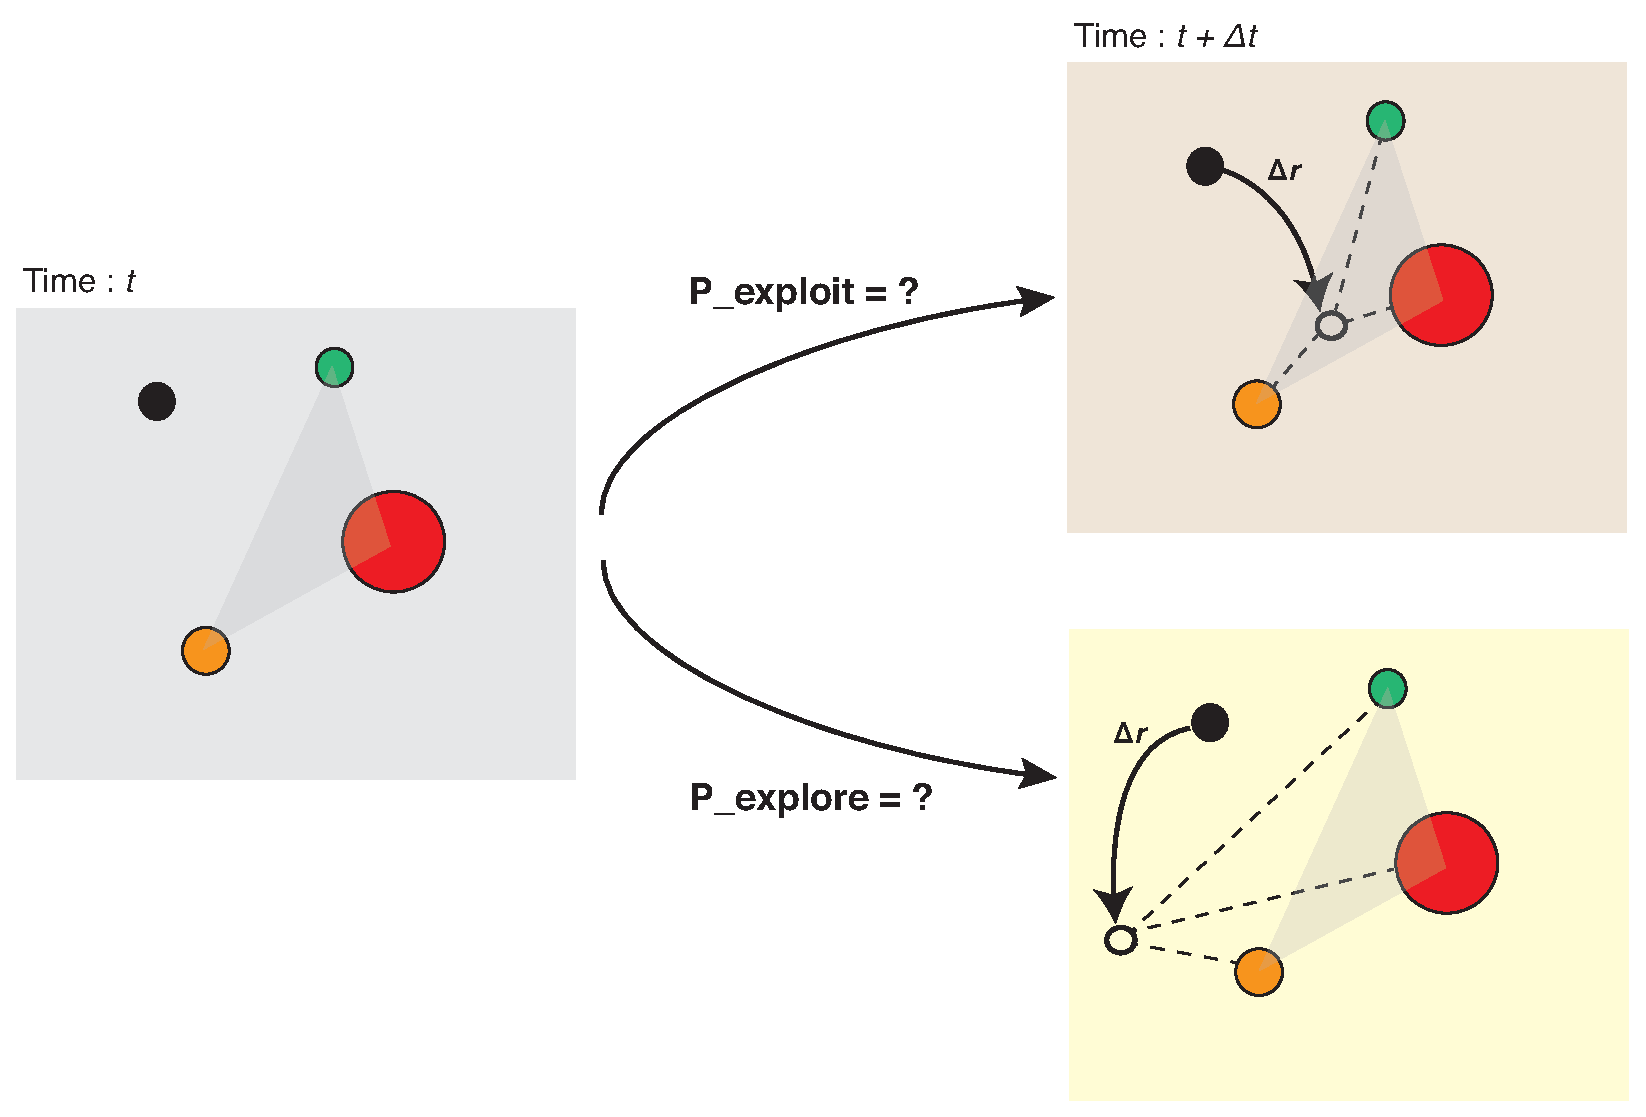
\includegraphics[width=10cm]{figures/schematic_displacement.eps}
\caption{2-dimensional schematic description of the {\it L\'evy flying mind} model ({\bf ``Proportional Attraction"}): At each time step, the individual must choose between remaining in the solution envelope that has already been explored and exploring outside the currently known solution envelope.  We assign some probability $p$ (a number between 0 and 1) to the participant's decision of staying in the explored envelop and probability $1-p$ to the decision to explore outside that envelop.  If it is harder to find solutions that offer a balanced re-combination of previous solutions than to think out-of-the-box and propose solutions outside of the current solution envelope, then $p < \frac{1}{2}$ else $p \geq \frac{1}{2}$.}
\label{fig:schematic}
\end{center}
\end{figure}










\subsection{Implications of Memory and Exploration on Performance}
Individuals deploy {\it exploration}, {\it exploitation}, and {\it return} strategies in order to get closer to the best solutions (i.e., factorizations of the joint distribution that are indistinguishable from the true model). Each move may lead to improvement (i.e., reduction of cognitive distance to the true model) or, on the contrary, to dis-improvement. 

We find that displacement has an influence on improvement. As one could surmise, small displacements can only bring marginal improvement, while larger displacements bring more opportunities for improvement, yet at the cost of potential short-term losses that may be quite large. Large displacements ($\Delta r > 0.2$) can bring rather negative performance. Figure \ref{fig:vs_dr} shows the evolution of the distance to the true model $D$ as a function of displacement $\Delta r$. The distance scales as $D \sim {\Delta r}^{\mu}$ with $\mu_{simple} = 0.88(1)$ [resp. $\mu_{complex} = 082(2)$]. For $\Delta r > 0.2$, $D$ uncertainty quickly balloons, but rather positive, reflecting the {\it cost} of making ``wild'' innovations. 

There is no clear relation between time spent on taking the decision to move and performance {\bf [show $\Delta D_{jsd}$ versus $\Delta t$] if relevant: question here is the functional form of how time spent on cognitive processing leads to better or worse results.}.

While there is no clear relation between time spent between moves and performance {\bf [$\Delta D_{jsd}$ versus $\Delta t$]}, the decision to make a larger displacement takes more time. For $\Delta r < 0.2$, the processing time before a displacement decision is made scales as $\Delta t \sim \Delta r^{\gamma}$ with $\gamma_{simple} = 0.11(1)$ [resp. $\gamma_{complex} = 0.13(1)$]. For $\Delta r > 0.2$, the processing times before a displacement decision is taken get disproportionally long (up to tens of seconds on average for a displacement of 0.7 (i.e., $\approx 25\%$ of the maximum displacement distance). On both panels, blue and red areas show the $25^{th}$ percentile confidence intervals.

The minimum distance $D_{min}$ (between the best model and the true model) exhibits a scaling as a function of the number of distinct sites visited $S_{T}$. $D_{min} \sim S_{T}^{\gamma}$ with resp. $\gamma_{simple} = -0.20(4)$ and $\gamma_{complex} = - 0.13(3)$. {\bf C.} The logarithm of number of visited sites is a linear function of the logarithm of time $t$. Hence, the number of distinct visited sites is a predictor of the minimum distance $D_{min}$ achieved at time $t$. The result also holds for groupings with averaged cognitive distances.


\begin{figure}[h!]
\begin{center}
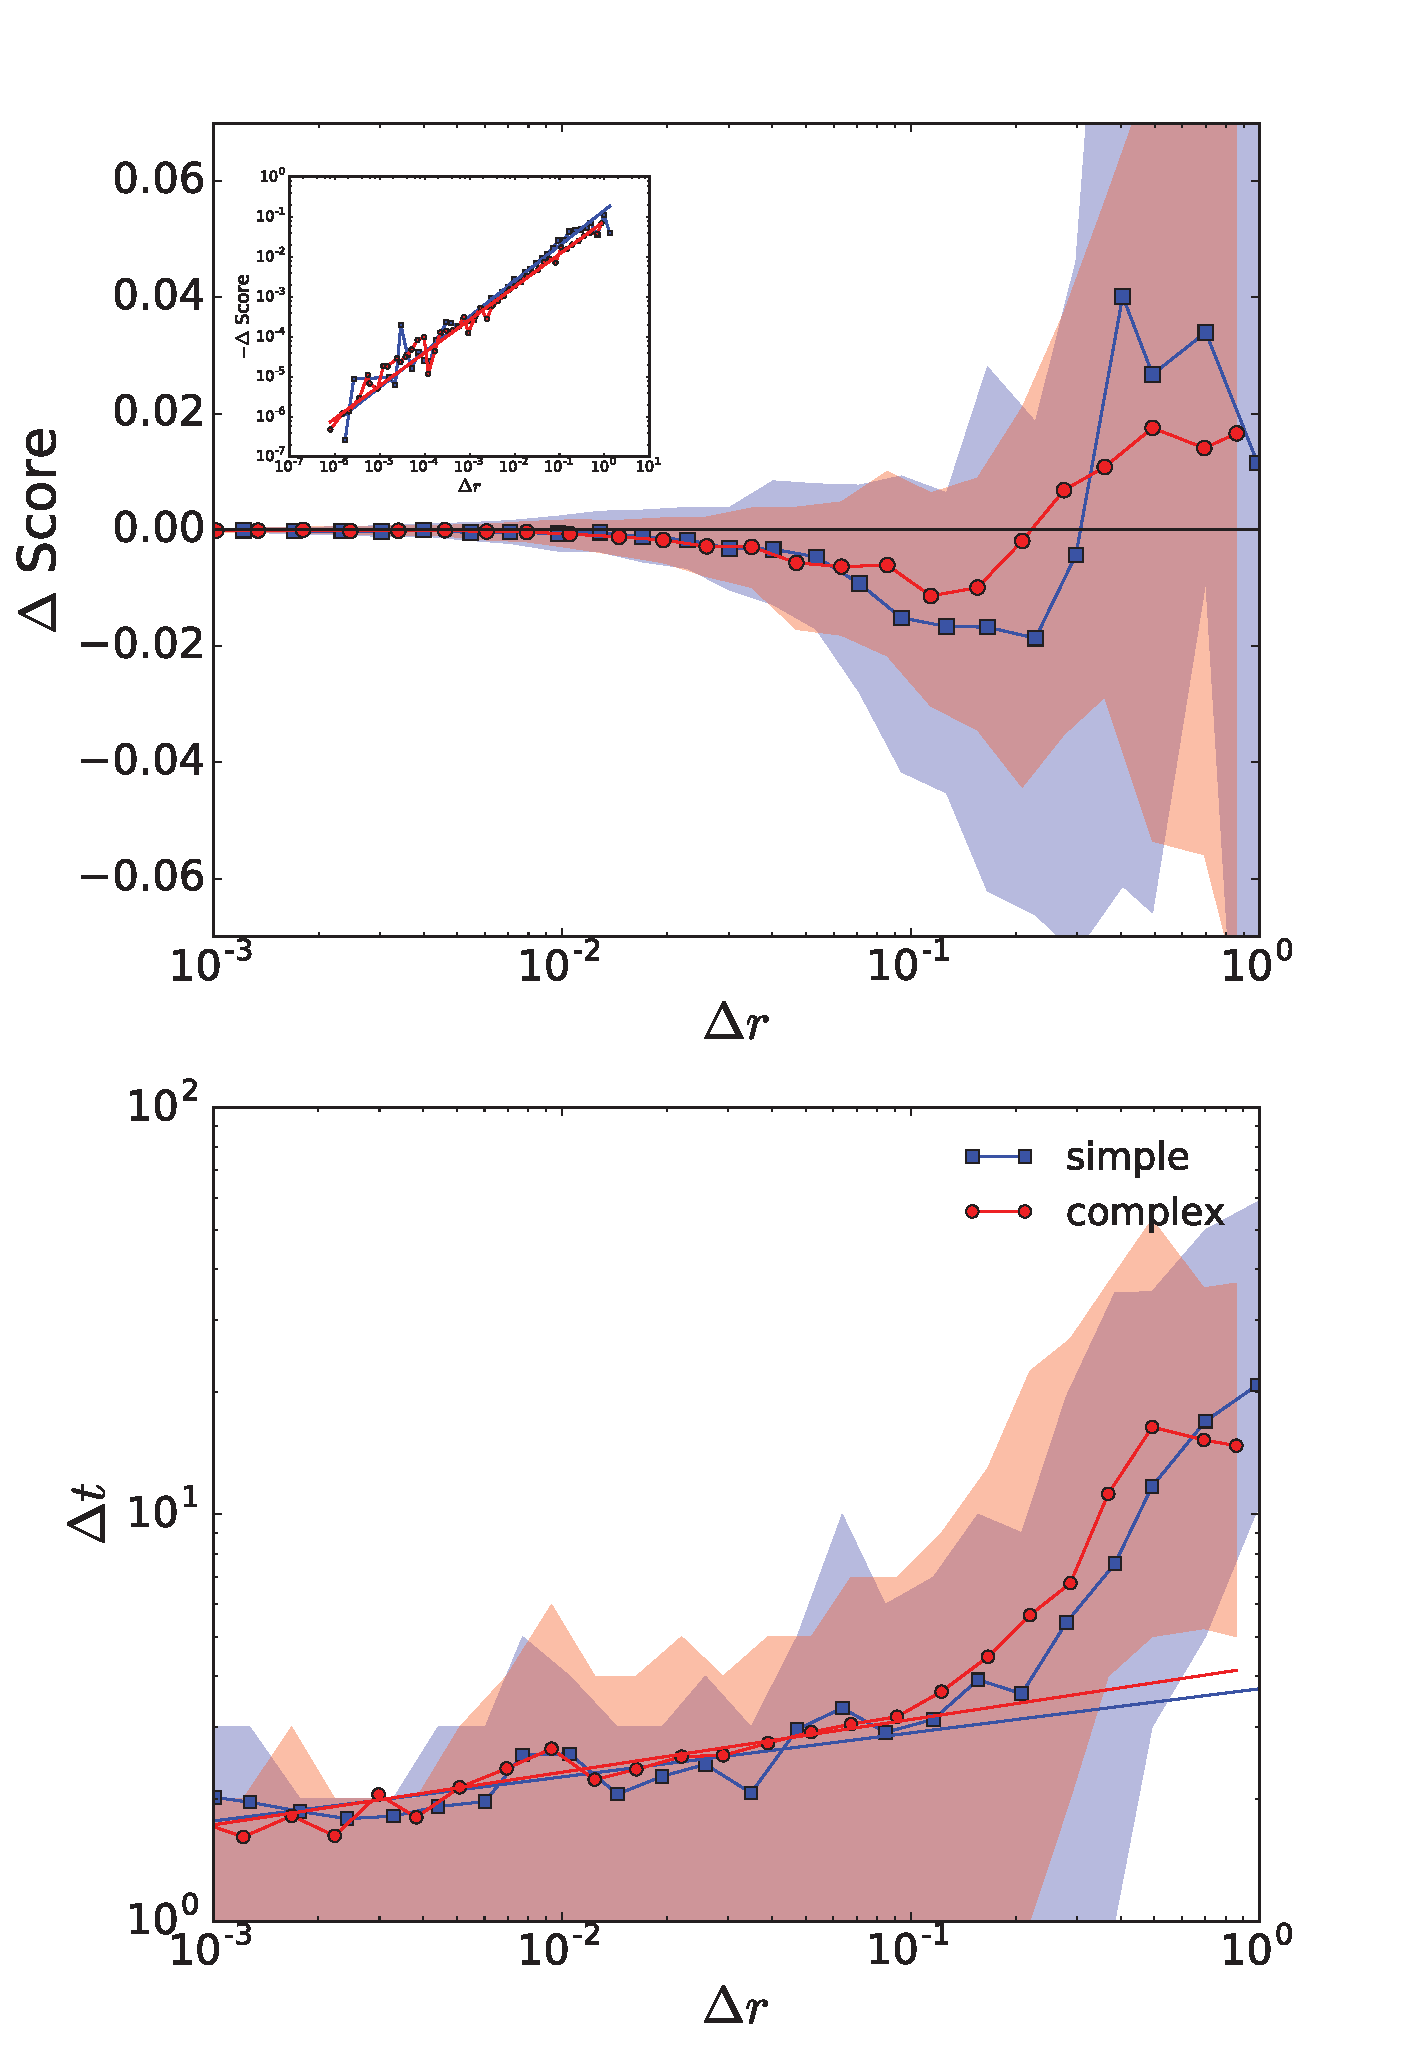
\includegraphics[width=11cm]{figures/vs_dr.eps}
\caption{{\bf A.} Evolution of the distance to the true model $D$ as a function of displacement $\Delta r$. The distance scales as $D \sim {\Delta r}^{\mu}$ with $\mu_{simple} = 0.88(1)$ [resp. $\mu_{complex} = 082(2)$]. For $\Delta r > 0.2$, $D$ becomes quickly highly uncertain, but rather positive, reflecting the {\it cost} of the making ``wild"displacements. {\bf B} For $\Delta r < 0.2$, the waiting time before a displacement decision is made scales as $\Delta t \sim \Delta r^{\gamma}$ with $\gamma_{simple} = 0.11(1)$ [resp. $\gamma_{complex} = 0.13(1)$]. For $\Delta r > 0.2$, the waiting time before a displacement decision is taken get disproportionally long (up to tens of seconds on average for displacement of 0.7 (i.e., $\approx 25\%$ of the maximum displacement distance). On both panels, blue and red areas show the 25th percentile confidence intervals.}.
%\caption{Scaling relation between $\Delta t$ and $\Delta r$ for the simple (A) and complex (B) treatments. The functions are similar for both treatments [resp. $\sim 0.44(2)$ ($p < 0.01$ , $r = 0.39$) and $\sim 0.47(2)$ ($p < 0.01$ , $r = 0.36$)]. {\bf Actually, one may see this figure differently : scaling $\Delta t \sim {\Delta r}^{0.2}$ for $\Delta r < 0.2$ and another (unknown) regime for $\Delta r > 0.2$ with waiting time getting disproportionately long $\rightarrow$ This may highlight the processing costs associated with a big jump.}}
\label{fig:vs_dr}
\end{center}
\end{figure}


\subsection{Computer vs. Optimal Foraging vs. Human Performance}

\begin{figure}[h!]
\begin{center}
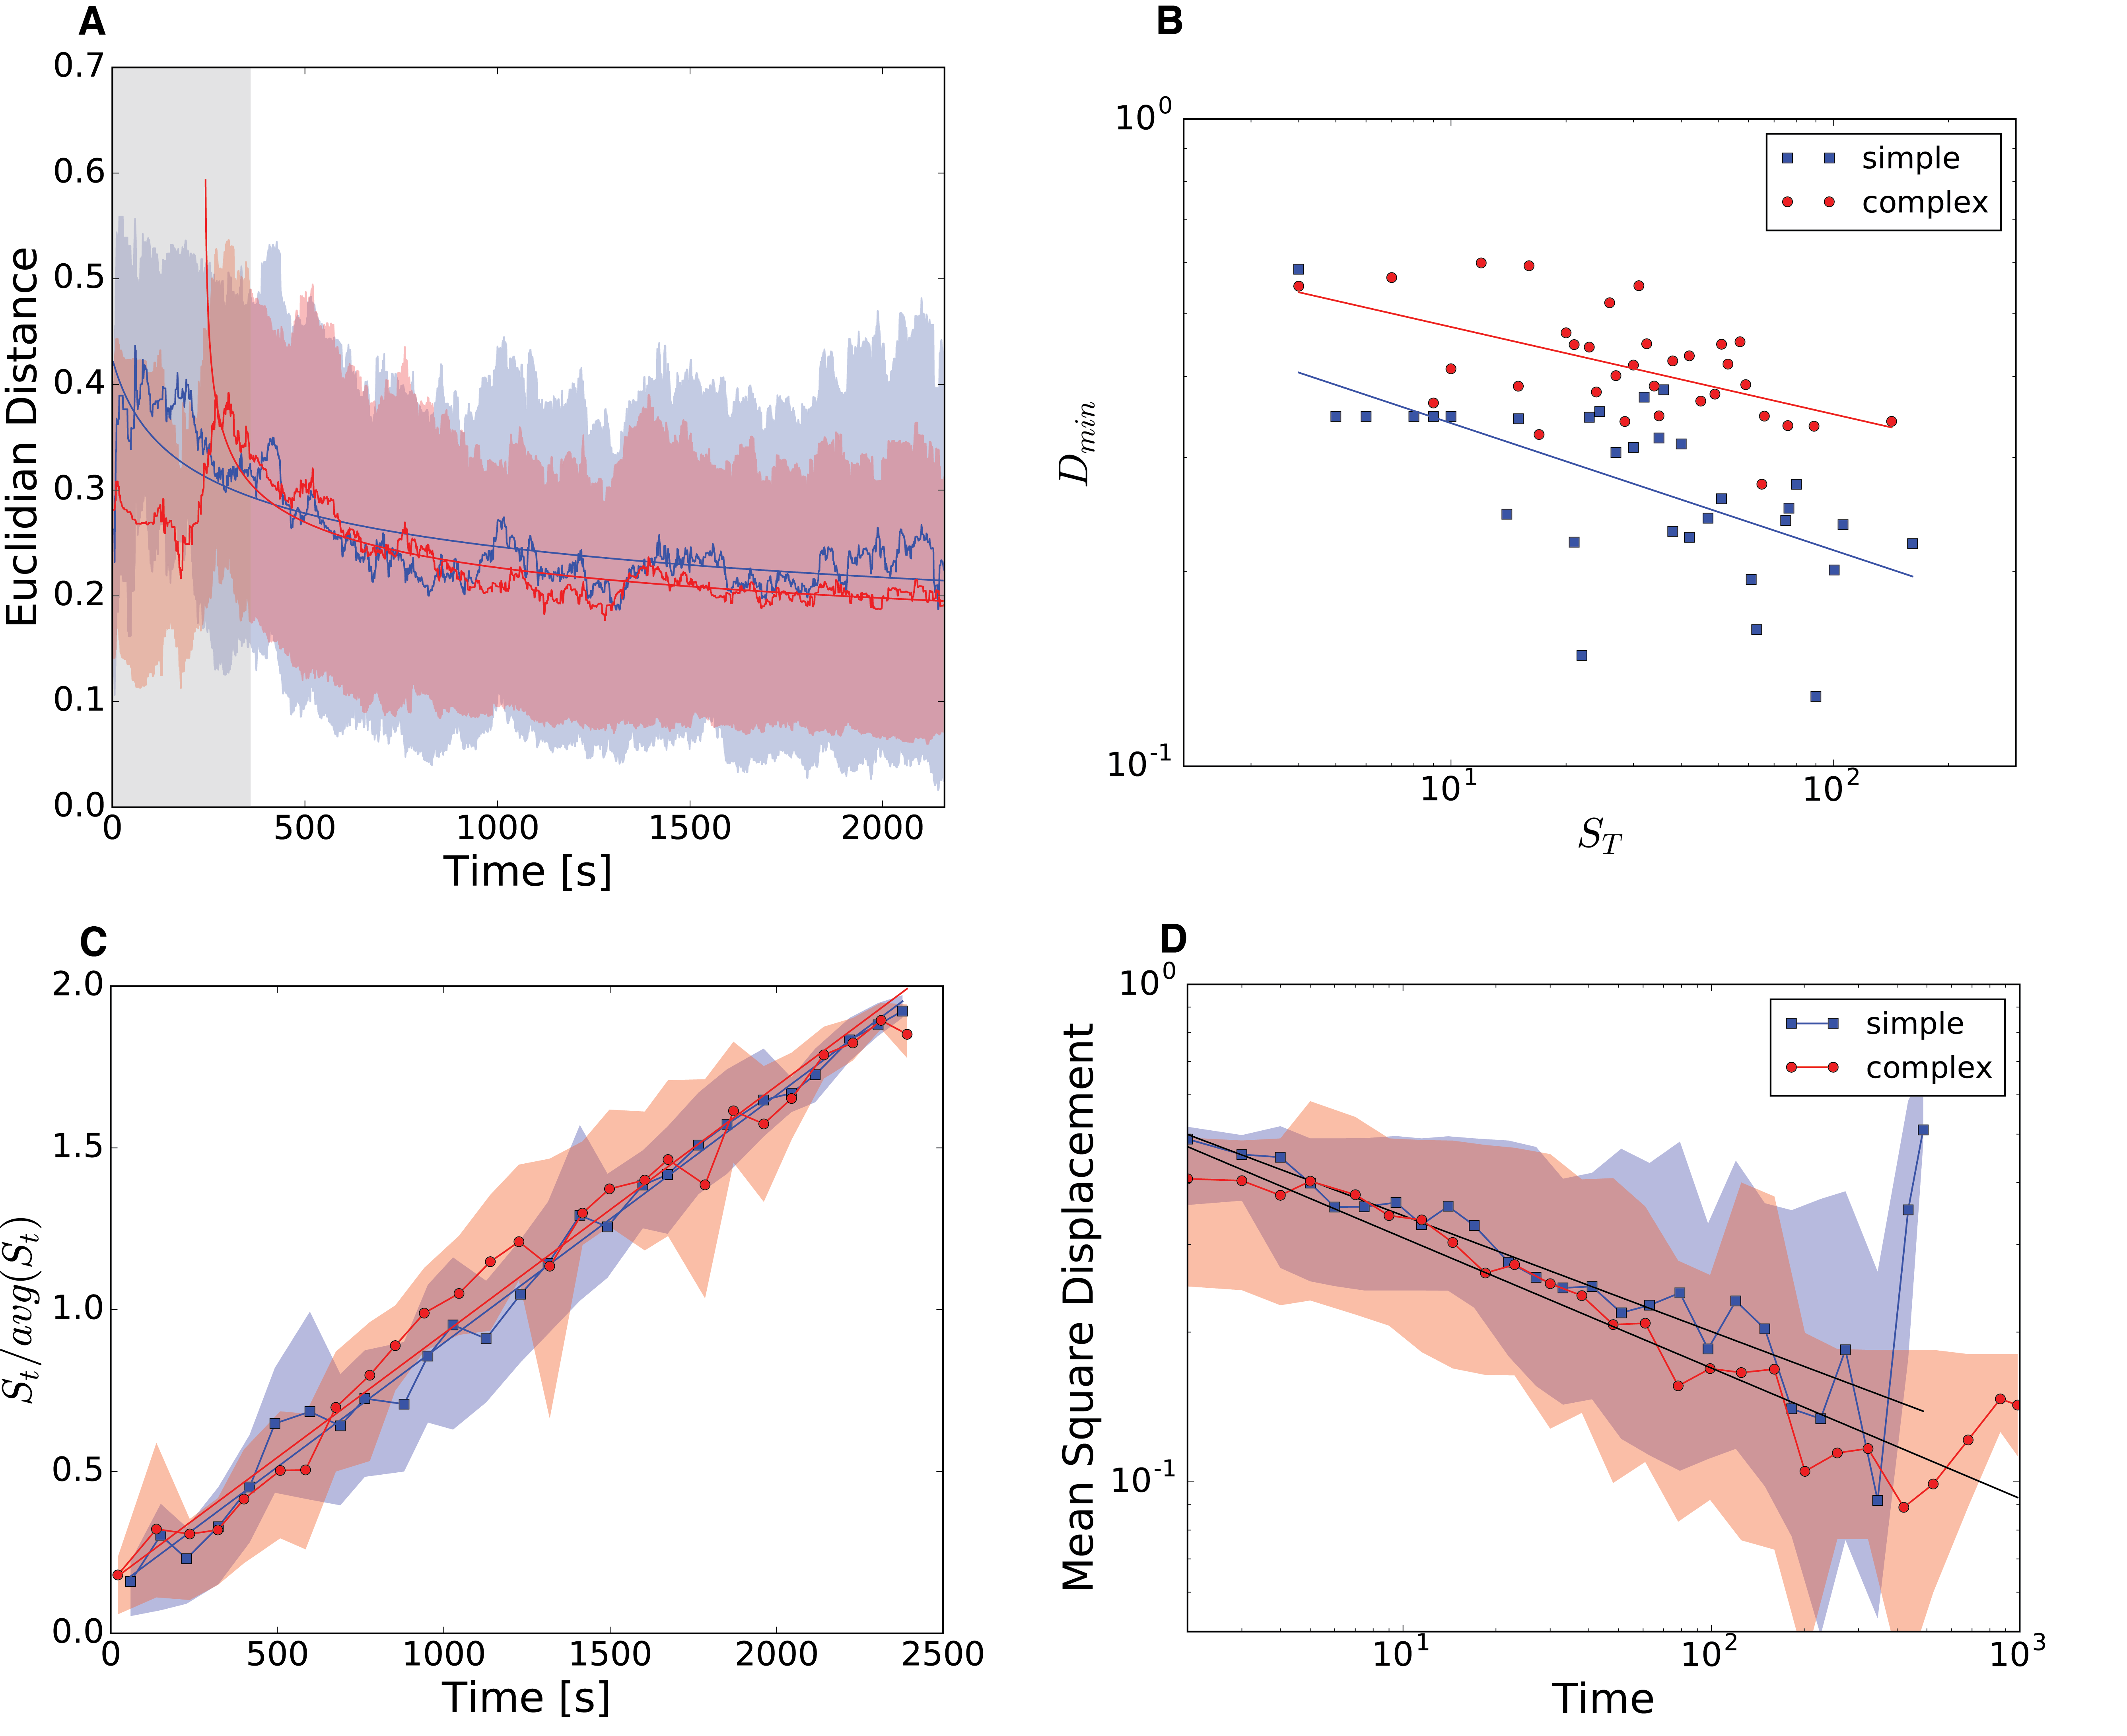
\includegraphics[width=16cm]{figures/Dmin_vs_St.eps}
\caption{{\bf A.} Minimum Euclidian distance $D_{min}$ (between the best model and the true model) exhibits a scaling as a function of the number of distinct sites visited $S_{T}$. $D_{min} \sim S_{T}^{\gamma}$ with resp. $\gamma_{simple} = -0.20(4)$ and $\gamma_{complex} = - 0.13(3)$. {\bf B.}  The number of visited sites over time $S_t$ is a linear function of time $t$. Hence, the number of distinct visited sites is a predictor of the minimum distance $D_{min}$ achieved. The result also holds for average distance. {\bf C.}  Mean square displacement (MSD) decays as $\sim t^{\mu}$ with $\mu_{simple} =-0.23(2)$ and $\mu_{complex} =- 0.26(1)$ showing a slow convergence (on the contrary of a normal L\'evy flight / CTRW, which is characterized by respectively diffusion $\mu_{Levy} = 1$ or super-diffusion $\mu_{CTRW} = \beta$ \cite{21,23}). All colored areas show the 25th percentile confidence intervals.}
\label{fig:Dmin_vs_St}
\end{center}
\end{figure}


{\bf [here, we should have a simulation of computer resolution process by a computer (Johannes you did this already), as well as a simulation of optimal foraging (displacement following a power law distribution with exponent 1)]}


\subsection{Waiting Times}

economic aspects (i.e., time is the scarce ressource)

\subsection{The Role of Incentives in Experimental Economics}

Experimental Economists have long differenciated themselves from experimenters in psychology and cognitive science, by rewarding their experimental participants directly for their efforts, such that better performance leads to higher expected payoffs from the laboratory experiment. The theories that are tested often mirror the conditions of a simplified but at least in one aspect realistic market environment and incentives are a natural and important part of such environments. It should be noted that outside of the laboratory, most cognitively demanding tasks have the characteristic that the quality of one's understanding is directly related to one's payoffs. This is true in the case of food search and it is true in the case of investment in a set of causally related securities, which the experiment from which we have our data seeks to mimic. Even in computational, agent based models, an agent must have some fitness or utility function that it has the intention to maximize \cite{dennett1989intentional} and in real human lives, money is theoretized to fulfill this fucntion well and this assumption has been tested in many other experiments and the evidence is largely consistent with this hypothesis.  The evidence has been summarized in a classic article \cite{smith1993} and the issue has been largely put to rest after that.    \cite{loewenstein99} gives a detailed critique on the external validity of experimental economics, where he acknowledges that some special institutions such as stock markets may be accurately represented through carefully structured experimental incentives. At the same time, the paper warns, some societal phenomena may not be well approximated enough through experimental economic methodology to have much external validity.   


\subsection{The Role of Incentives in our specific experiment}

The Becker-Degroot Marshak Method, in particular, is a workhorse in experimental economics, as a true valuation revealing incentive scheme for random goods \cite{ortega2018mitigating, tymula2016flexible, diro2016effect}. 
They way that this works is that a lottery is defined; in our case the lottery is that if some variable will take on the value H then playing the lottery will have a payoff of \$ 1 and if the variable takes on the value L, playing the lottery will payoff \$ 0.  In our case, whatever value the variable takes on is probabilistically determined by whatever values two or three covariates have already taken on and those values, but not their probabilistic influences, are known.  So, conditional on some other variables' known values, the lotery is regarding the hidden value of some variable.  Now, given our lotery, the Becker-Degroot Marshak Method is as follows.  Participants are stating in essence what they believe this lottery is worth.  By stating, for example, through their setting of parameters, that the probability of the variable taking on H is 0.5, then this is the same as stating that the lottery is worth \$ 0.5.  Then the computer decides an offer price and if this price is \$ 0.6, the participant is immediately rewarded 60 cents, however if this random offer price is 40 cents, then the participant ends up playing the lottery and is awarded \$ 1 if the variable takes on the value H and otherwise \$ 0.  This incentive scheme has been shown to be truth revealing of peoples beliefs regarding the value of some good (any good) and in particular the believed value (in this case just the probability expressed in cents) of some lottery.  Since this is repeated 30 times, at maximum stake are 30 dollars and everage payoffs were around \$14.  A \$ 5 dollar showup fee was also paid, so average total take-home pay for the participants was \$ 19.    

\cite{irwing98} empirically shows that steep incentive differences for better results might be necessary for cases in which individuals must seek out the solution to a problem and in which it isn't easy to deduce.  How steep are the differences in incentives in our experiment, are they steep enough, given the complexity of the problem at hand?  We can not definitively answer that question and through cognitive cost explanations the slow learning might be partially or in total a result of not sufficiently steep incentive differences. More work would be needed to know if it is the insufficiently steep incentives or the sufficiently steep cognitive costs that determine the characteristics of the learning curve in our experiment.     
